% !TEX root = ../tex/3-4.tex
% 第3章：本文は青、補足は緑
\newcommand{\asmain}{%
    \setbeamercolor{frametitle}{fg=white,bg=main}%
    \setbeamercolor{structure}{fg=main}%
    \setbeamercolor{itemize item}{fg=main}%
    \setbeamercolor{itemize subitem}{fg=main}%
    \setbeamercolor{enumerate item}{fg=main}%
}
\newcommand{\assuppl}{%
    \setbeamercolor{frametitle}{fg=white,bg=examplecol}%
    \setbeamercolor{structure}{fg=examplecol}%
    \setbeamercolor{itemize item}{fg=examplecol}%
    \setbeamercolor{itemize subitem}{fg=examplecol}%
    \setbeamercolor{enumerate item}{fg=examplecol}%
}
\asmain


%=============================================
\begin{frame}{3.3から3.4へ}
    \begin{block}{ここまで（3.3）}
        単一ノイズのDSMで、条件付きスコアを教師にして
        周辺分布のスコアを学習できる。\\
        Tweedieの公式により、スコア予測とノイズ除去が結びつく。
    \end{block}
    \begin{block}{ここから（3.4）}
        ノイズが1段階だけだと、粗さ・細かさ・モード横断を同時には満たせない。\\
        複数ノイズでスコアを条件付き学習し、
        アニーリングしたランジュバンで生成する（NCSN）。
    \end{block}
\end{frame}
%=============================================
\asmain
\begin{frame}{3.4 の位置づけ}
    \begin{block}{この節の役割}
        単一ノイズのDSMを、複数ノイズのNCSNへ拡張する
    \end{block}
    \begin{enumerate}
        \item \textbf{3.4.1 動機}\\
        単一ノイズの限界と、複数ノイズ＋アニーリングの発想
        \item \textbf{3.4.2 学習}\\
        ノイズ条件付きスコアネットと損失（3.4.1）、DDPMとの対応
        \item \textbf{3.4.3 サンプリング}\\
        Annealed Langevin Dynamicsと、遅い理由
    \end{enumerate}
    \vfill
    \footnotesize
    Song and Ermon (2019)
\end{frame}
%=============================================
\section{3.4.1 動機}
\asmain
\begin{frame}{区切り：3.4.1 動機}
    \tableofcontents[currentsection]
\end{frame}
%=============================================
\asmain
\begin{frame}{単一ノイズでは足りない}
    固定分散のガウスノイズを1つだけ入れると、分布はある程度滑らかになる。\\
    しかし、ノイズレベルを1つに固定すると次の限界が出る。
    \begin{columns}[T,onlytextwidth]
        \begin{column}{0.48\textwidth}
            \begin{block}{低ノイズ}
                細部は残るが、低密度領域で勾配が弱く、
                多峰分布のモード間を渡りにくい。
            \end{block}
        \end{column}
        \begin{column}{0.48\textwidth}
            \begin{block}{高ノイズ}
                探索はしやすいが、粗い構造しか捉えられず、
                ぼけたサンプルになりやすい。
            \end{block}
        \end{column}
    \end{columns}
    \vfill
    高次元では、初期化が悪いとプラトーや鞍点付近で探索が止まり、
    一つのモードに閉じ込もり得る。
\end{frame}
%=============================================
\asmain
\begin{frame}{図3.6：低密度ではスコア推定が不安定}
    \centering
    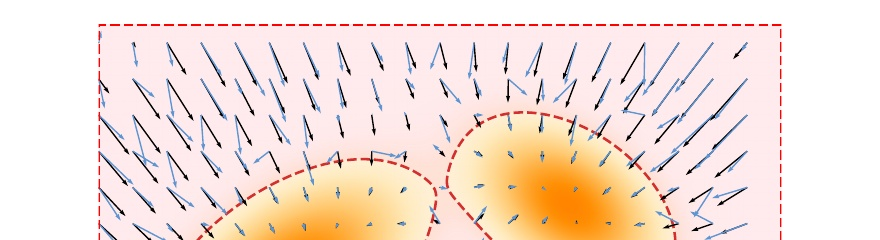
\includegraphics[width=\textwidth,height=0.68\textheight,keepaspectratio]{fig-3-6.jpg}
    \vfill
    赤の領域はサンプルが少なく、スコア推定が不正確になりやすい。\\
    高密度側では推定が比較的安定する。
\end{frame}
%=============================================
\assuppl
\begin{frame}{\supplmark：図3.6の読み方}
    \begin{exampleblock}{オレンジの島}
        データの高密度領域である。\\
        ここでのスコアは、サンプルが多いため比較的信じやすい。
    \end{exampleblock}
    \begin{exampleblock}{赤い低密度領域}
        観測が薄いので、スコアマッチングの誤差が大きくなりやすい。\\
        ランジュバンがモード間を渡るときに通る場所でもある。
    \end{exampleblock}
    \begin{exampleblock}{単一ノイズの難しさ}
        細部を残す低ノイズでは、この低密度の壁が残りやすい。\\
        壁を消す高ノイズでは、細部が潰れる。
    \end{exampleblock}
\end{frame}
%=============================================
\asmain
\begin{frame}{複数ノイズとアニーリングで両方を取る}
    Song and Ermon (2019) は、複数レベルのガウスノイズを入れ、
    ノイズ条件付きスコアネット（NCSN）をまとめて学習する。
    \begin{block}{生成時}
        ノイズをアニーリングするランジュバン動力学を使う。
        \begin{itemize}
            \item 高ノイズ：粗い探索でモード間を渡りやすくする
            \item 低ノイズ：細部を復元する
        \end{itemize}
    \end{block}
    \begin{itemize}
        \item 学習：$s_\phi(\bm{x},\sigma)$を多くの$\sigma$で同時に当てる
        \item 生成：大きい$\sigma$から小さい$\sigma$へ段階的に移る
    \end{itemize}
\end{frame}
%=============================================
\asmain
\begin{frame}{図3.7：NCSNの流れ}
    \centering
    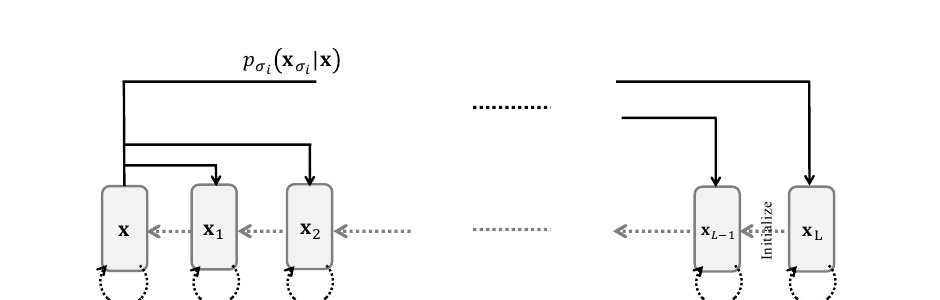
\includegraphics[width=\textwidth,height=0.62\textheight,keepaspectratio]{fig-3-7.jpg}
    \vfill
    前方は複数ノイズ$p_{\sigma}(\bm{x}_{\sigma}|\bm{x})$でデータを崩す。\\
    生成（破線）は各ノイズでランジュバンし、次のより低いノイズの初期値にする。
\end{frame}
%=============================================
\assuppl
\begin{frame}{\supplmark：図3.7の読み方}
    \begin{columns}[T,onlytextwidth]
        \begin{column}{0.48\textwidth}
            \begin{exampleblock}{上向きの実線}
                きれいな$\bm{x}$から、
                各ノイズレベル$\sigma_i$の
                $\bm{x}_i$を作る前向き過程。
            \end{exampleblock}
        \end{column}
        \begin{column}{0.48\textwidth}
            \begin{exampleblock}{破線の右$\to$左}
                $\bm{x}_L$から$\bm{x}$へ戻る生成。\\
                各段の下のループが、
                そのノイズでのランジュバン更新。
            \end{exampleblock}
        \end{column}
    \end{columns}
    \vspace{0.4em}
    \begin{exampleblock}{Initialize}
        あるノイズ段の最終状態を、
        ひとつ小さいノイズ段の初期値にする。\\
        これがアニーリングの本体である。
    \end{exampleblock}
\end{frame}
%=============================================
\asmain
\begin{frame}{3.4.1 のまとめ}
    \begin{itemize}
        \item 単一ノイズでは、細部保存とモード横断を両立しにくい
        \item 低密度ではスコア推定が不安定になりやすい（図3.6）
        \item NCSNは複数ノイズで学習し、高$\to$低へアニーリングして生成する
    \end{itemize}
    \begin{block}{次}
        複数ノイズでの学習目的関数を書く。
    \end{block}
\end{frame}
%=============================================
\section{3.4.2 学習}
\asmain
\begin{frame}{区切り：3.4.2 学習}
    \tableofcontents[currentsection]
\end{frame}
%=============================================
\asmain
\begin{frame}{複数のノイズレベルを用意する}
    ノイズ列$\{\sigma_i\}_{i=1}^{L}$を
    \[
        0<\sigma_1<\sigma_2<\cdots<\sigma_L
    \]
    となるように選ぶ。
    \begin{itemize}
        \item $\sigma_1$：細部がほぼ残る程度に小さい
        \item $\sigma_L$：分布が十分滑らかになる程度に大きい
    \end{itemize}
    各ノイズでは、きれいなデータ$\bm{x}\sim p_{\mathrm{data}}$に
    \[
        \bm{x}_{\sigma}
        =
        \bm{x}+\sigma\bm{\epsilon},
        \qquad
        \bm{\epsilon}\sim\mathcal{N}(\bm{0},\bm{I})
    \]
    を加える。
\end{frame}
%=============================================
\asmain
\begin{frame}{摂動核と周辺分布}
    \begin{block}{摂動核}
        \[
            p_{\sigma}(\bm{x}_{\sigma}|\bm{x})
            :=
            \mathcal{N}(\bm{x}_{\sigma};\,\bm{x},\,\sigma^{2}\bm{I})
        \]
    \end{block}
    \begin{block}{周辺分布}
        \[
            p_{\sigma}(\bm{x}_{\sigma})
            =
            \int
            p_{\sigma}(\bm{x}_{\sigma}|\bm{x})\,
            p_{\mathrm{data}}(\bm{x})\,
            d\bm{x}
        \]
        各$\sigma$での、ガウス平滑化されたデータ分布である。
    \end{block}
\end{frame}
%=============================================
\asmain
\begin{frame}{NCSNの学習目的}
    ノイズ条件付きスコアネット$s_\phi(\bm{x},\sigma)$で、
    すべての$\sigma\in\{\sigma_i\}_{i=1}^{L}$について
    $\nabla_{\bm{x}}\log p_{\sigma}(\bm{x})$を推定する。
    \[
        \mathcal{L}_{\mathrm{NCSN}}(\phi)
        :=
        \sum_{i=1}^{L}
        \lambda(\sigma_i)\,
        \mathcal{L}_{\mathrm{DSM}}(\phi;\sigma_i)
        \tag{3.4.1}
    \]
    ここで$\lambda(\sigma_i)>0$は各スケールの重みである。
    \[
        \resizebox{0.98\textwidth}{!}{$
        \mathcal{L}_{\mathrm{DSM}}(\phi;\sigma)
        =
        \dfrac12
        \mathbb{E}_{\bm{x}\sim p_{\mathrm{data}},\,
        \tilde{\bm{x}}\sim p_{\sigma}(\cdot|\bm{x})}
        \Bigl\|
        s_\phi(\tilde{\bm{x}},\sigma)
        -
        \dfrac{\bm{x}-\tilde{\bm{x}}}{\sigma^{2}}
        \Bigr\|_{2}^{2}
        $}
    \]
\end{frame}
%=============================================
\assuppl
\begin{frame}{\supplmark：単一DSMの和になっている}
    各$\sigma_i$での$\mathcal{L}_{\mathrm{DSM}}$は3.3のDSMそのものである。\\
    教師は条件付きスコア
    $\nabla_{\tilde{\bm{x}}}\log p_{\sigma}(\tilde{\bm{x}}|\bm{x})=(\bm{x}-\tilde{\bm{x}})/\sigma^{2}$。
    \begin{exampleblock}{最適解}
        定理3.3.1より、各ノイズで
        \[
            s^{\star}(\cdot,\sigma)
            =
            \nabla_{\bm{x}}\log p_{\sigma}(\cdot)
        \]
        が得られる。NCSNはそれを全$\sigma_i$で同時に求める。
    \end{exampleblock}
\end{frame}
%=============================================
\asmain
\begin{frame}{DDPM損失との関係}
    $\bm{x}_{\sigma}=\bm{x}+\sigma\bm{\epsilon}$とし、Tweedieより
    \[
        \nabla_{\bm{x}_{\sigma}}\log p_{\sigma}(\bm{x}_{\sigma})
        =
        -\frac{1}{\sigma}\,\mathbb{E}[\bm{\epsilon}|\bm{x}_{\sigma}]
    \]
    したがって
    \[
        s^{\star}(\bm{x}_{\sigma},\sigma)
        =
        -\frac{1}{\sigma}\,\bm{\epsilon}^{\star}(\bm{x}_{\sigma},\sigma),
        \qquad
        \bm{\epsilon}^{\star}(\bm{x}_{\sigma},\sigma)
        =
        -\sigma\,s^{\star}(\bm{x}_{\sigma},\sigma)
    \]
    \begin{block}{読み方}
        DDPMの最適ノイズ予測と、NCSNの最適スコアは、
        既知のスケール$1/\sigma$を除いて同じ情報をもつ。
    \end{block}
\end{frame}
%=============================================
\assuppl
\begin{frame}{\supplmark：DDPMのステップ表記との対応}
    DDPMでは
    \[
        \sigma_i:=\sqrt{1-\bar{\alpha}_i^{2}},
        \qquad
        \bm{x}_i=\bar{\alpha}_i\bm{x}_0+\sigma_i\bm{\epsilon}
    \]
    と書ける。このとき
    \[
        s^{\star}(\bm{x}_i,i)
        =
        -\frac{1}{\sigma_i}\,\mathbb{E}[\bm{\epsilon}|\bm{x}_i]
    \]
    \begin{exampleblock}{要点}
        ステップ$i$でのノイズ予測は、
        ノイズレベル$i$でのスコア予測と等価である
        （係数$1/\sigma_i$を除く）。\\
        系統的な比較は第6章に回す。
    \end{exampleblock}
\end{frame}
%=============================================
\asmain
\begin{frame}{3.4.2 のまとめ}
    \begin{itemize}
        \item 複数ノイズ$0<\sigma_1<\cdots<\sigma_L$でDSMを足し合わせる（3.4.1）
        \item ネットは$s_\phi(\bm{x},\sigma)$としてノイズを条件に取る
        \item 最適スコアとDDPMの最適ノイズ予測は$1/\sigma$で互いに移る
    \end{itemize}
    \begin{block}{次}
        学習した複数スコアを、アニーリング・ランジュバンで使う。
    \end{block}
\end{frame}
%=============================================
\section{3.4.3 サンプリング}
\asmain
\begin{frame}{区切り：3.4.3 サンプリング}
    \tableofcontents[currentsection]
\end{frame}
%=============================================
\asmain
\begin{frame}{Annealed Langevin Dynamics}
    学習済みスコア
    $s_{\phi^\star}(\cdot,\sigma_1),\ldots,s_{\phi^\star}(\cdot,\sigma_L)$
    を使い、
    大きいノイズ$\sigma_L$から小さいノイズ$\sigma_1\approx 0$へ進む。
    \begin{enumerate}
        \item $\bm{x}\sim p_{\mathrm{init}}$（最大ノイズ向けの雑な初期分布）
        \item $\ell=L,L-1,\ldots,1$について：
        \begin{itemize}
            \item 前段の出力を初期値$\tilde{\bm{x}}_0\leftarrow\bm{x}$にする
            \item $\sigma_\ell$でランジュバンを$N_\ell$回回す
            \item 最終状態を次段へ渡す
        \end{itemize}
    \end{enumerate}
    最終的に最小ノイズ$\sigma_1$での洗練を経た$\bm{x}$を出力する。
\end{frame}
%=============================================
\asmain
\begin{frame}{各ノイズでの更新則}
    ノイズレベル$\sigma_\ell$では
    \[
        \tilde{\bm{x}}_{n+1}
        =
        \tilde{\bm{x}}_n
        +
        \eta_\ell\,s_{\phi^\star}(\tilde{\bm{x}}_n,\sigma_\ell)
        +
        \sqrt{2\eta_\ell}\,\bm{\epsilon}_n,
        \qquad
        \bm{\epsilon}_n\sim\mathcal{N}(\bm{0},\bm{I})
    \]
    ステップ幅の典型例は
    \[
        \eta_\ell
        =
        \delta\,\frac{\sigma_\ell^{2}}{\sigma_1^{2}},
        \qquad
        \delta>0
    \]
    \begin{block}{要点}
        ノイズが大きいほどステップを大きく取り、
        ノイズが小さくなるほど細かく動かす。
    \end{block}
\end{frame}
%=============================================
\assuppl
\begin{frame}{\supplmark：アルゴリズムの骨格}
    \footnotesize
    \begin{enumerate}
        \item $\bm{x}\sim p_{\mathrm{init}}$
        \item \textbf{for} $\ell=L,L-1,\ldots,1$ \textbf{do}
        \begin{enumerate}
            \item $\tilde{\bm{x}}_0\leftarrow\bm{x}$
            \item \textbf{for} $n=0,\ldots,N_\ell-1$ \textbf{do}
            \begin{enumerate}
                \item $\bm{\epsilon}_n\sim\mathcal{N}(\bm{0},\bm{I})$
                \item
                $\tilde{\bm{x}}_{n+1}\leftarrow
                \tilde{\bm{x}}_n
                +\eta_\ell s_{\phi^\star}(\tilde{\bm{x}}_n,\sigma_\ell)
                +\sqrt{2\eta_\ell}\,\bm{\epsilon}_n$
            \end{enumerate}
            \item $\bm{x}\leftarrow\tilde{\bm{x}}_{N_\ell}$
        \end{enumerate}
        \item 出力$\bm{x}$
    \end{enumerate}
    \normalsize
    \begin{exampleblock}{読み方}
        外側のループがノイズのアニーリング、
        内側のループがそのノイズでのMCMCである。
    \end{exampleblock}
\end{frame}
%=============================================
\asmain
\begin{frame}{NCSNのサンプリングは遅い}
    各ノイズ$\sigma_i$で、スコア評価＋微小ノイズの更新を$K$回繰り返す。\\
    全体でおおよそ$L\times K$回の順次ネット評価が要る。
    \begin{columns}[T,onlytextwidth]
        \begin{column}{0.48\textwidth}
            \begin{block}{(i) 局所精度}
                学習したスコアは小さな摂動向きに信頼できる。\\
                ステップを小さくし、段ごとに多数回回す必要がある。
            \end{block}
        \end{column}
        \begin{column}{0.48\textwidth}
            \begin{block}{(ii) 混合の遅さ}
                高次元・多峰では局所的なMCMC移動が非効率で、
                典型領域へ届くまで反復が増える。
            \end{block}
        \end{column}
    \end{columns}
    \vfill
    更新は直前状態に依存し並列化しにくいので、計算コストは$\mathcal{O}(LK)$になる。
\end{frame}
%=============================================
\asmain
\begin{frame}{3.4.3 のまとめ}
    \begin{itemize}
        \item 生成は高ノイズから低ノイズへ、段ごとにランジュバンする
        \item 前段の出力が次段の初期値になる（アニーリング）
        \item 段数$\times$段内反復のため、サンプリングは計算的に重い
    \end{itemize}
\end{frame}
%=============================================
\asmain
\begin{frame}{3.4 全体のまとめ}
    \begin{enumerate}
        \item \textbf{動機}
        単一ノイズでは粗さ・細部・モード横断を同時に満たせない。
        \item \textbf{学習}
        $s_\phi(\bm{x},\sigma)$を複数$\sigma$のDSM和（3.4.1）で学ぶ。\\
        DDPMのノイズ予測とは$1/\sigma$で等価。
        \item \textbf{生成}
        Annealed Langevinで$\sigma_L\to\sigma_1$と洗練する。
        \item \textbf{課題}
        $\mathcal{O}(LK)$の順次評価によりサンプリングが遅い。
    \end{enumerate}
\end{frame}
%=============================================
\asmain
\begin{frame}{3.4 全体のまとめ：一本の流れ}
    \begin{block}{今日の道筋}
        単一ノイズの限界
        $\;\to\;$
        複数ノイズでスコアを条件付き学習
        $\;\to\;$
        高$\to$低へアニーリング生成
        $\;\to\;$
        ただしMCMCが重い
    \end{block}
    \begin{block}{核心}
        NCSNは「どのくらい崩れた分布のスコアか」を$\sigma$で条件付け、
        粗い探索から細部復元へ段階的に戻す。
    \end{block}
    \begin{block}{次へ}
        3.5ではNCSNとDDPMを表で比較し、共通点と違いを整理する。
    \end{block}
\end{frame}
